\chapter{Introduction}

\section{Motivation for Twisted van der Waals Materials}
The main topic of condensed matter physics are about phases and phase transitions. In this thesis, we focus on the study of zero-temeprature phases and transitions, i.e., the \emph{quantum} phases of matter and \emph{quantum} phase transtions.

From the perspective of experiments, these two topics roughly corresponds the two main strategies in search of exotic quantum phases of matter:
\begin{itemize}
    \item one way is to directly step into the quantum phases by growing new materials;
    \item the other one is to drive phase tansitions from existing materials by tune external parameters.
\end{itemize}
Traditionally the former way is more popular due to the variaty and maturity of the material growth techniques and experimental apparatus. For example, iron-based superconductors FeSe thin films are grown with MBE (Molecular Beam Epitaxy) \cite{lee2014interfacial}, the cuprates like YBa$_2$Cu$_3$O$_{7-x}$ are grown with PLD (Pulsed Laser Deposition) \cite{roas1988epitaxial}, and the Kitaev candidate $\alpha$-RuCl$_3$ are grown with CVT (Chermial Vapor Transport) \cite{gronke2018chemical}. However, the drawback of the material-growth strategy is that it is hard to connect the lattice-level information, including the lattice constants, bond angles, the doppings with the material properties to the mesoscopic physical properties of the grown materials, and the growth procedure itself is always a time-consuming, expensive, and labor-intensive process. As for the other way, there are plenty of external parameters that can be tuned, like dopping, pressure, magnetic field, gating field, and so on. The advantage over the material-growth route is its tunability and controllability. For example, fractional quantum Hall effect (FQHE) is disordered by turning on a large magnetic fields in very clean GaAs/AlGaAs heterostructures \cite{tsui1982two,willett1987observation,stormer1999fractional}, and the high-pressure room-temeprature superconductors are obtained by tunning the pressure up to 200 GPa \cite{gor2018colloquium}. However, there are still drawback for the parameter-tuning strategy: usually the entire phase diagram is unknown to us, and there can be many competing phases close to the target phase. More seriously, to reach some exotic phases, the parameter has been tuned to some extreme value that is really hard to achieve for most experimental groups, and we may fall back to the old problem of the high expenses.


So a natural problem is to ask that how to \emph{effectively} search and explore the exotic quantum phase of matters, or more precisely can we find a platform combinating both experimental routes' advantages but avoid their drawbacks? Here ``effective'' can be understood as many aspects: the cost, the time consumption, the labor, the predictability, the controllability, and so on. It turns out that, the rapidly growing fields of \emph{twisted physics}, or \emph{twistronics}, provides an answer to this question.


In study of twisted physics, at least two layers of building blocks are stacked together, stablizing with weak interlayer van der Waals interactions (so are also called \emph{van der Waals (vdW) materials}) with the presence of some twisting angles. It has been commonly agreed that most of these 2D materials are cheap for exfoliation and fabrication (and can be easier in comparison with material growth approach). The familiar tuning parameters like magnetic fields/gating fields can still be used here. The advantage of twisted physics is that, the number of stacking layers, as well as the twist angle between each two layers, can be recognized as a new experimental knob to tune the electronic properties of the system, which is also fully controllable and tunable.

\subsection{On Dimensionality}
The building blocks in twisted physics are mainly graphene, transition metal dichalcogenides (TMD), and other two-dimensional (2D) materials including monolayer cuprates and monolayer iron-based superconductor FeSe. Reducing the dimensionality of a system is believed to be associated with enhancement of the quantum effects. In fact, before the discovery of monolayer graphene in 2004 by Geim and Novoselov \cite{novoselov2004electric}, people even wrongly use the entropy argument, or Mermin-Wagner theorem to argue the non-existence of 2D materials, and even Lev Landau made mistakes here\footnote{Landau claim the non-existence based on the experimental facts that no divergence has been observed under a disorder to order (like liquid to crystal) phase transition. But most arguments are wrong here due to the presence of lattice structure and the absence of divergence.}. But nowadays, we know that a vast family of 2D materials has been grown, including metals like NbSe$_2$ \cite{tsen2016nature}, semi-conductor like most TMD materials \cite{manzeli20172d}, insulators like hexagonal Boron nitride (hBN), and even 2D magnets like CrI$_3$ \cite{huang2017layer,huang2018electrical}. The broadening of the 2D materials family opened up the possibility to stack different 2D crystals on top of each other thus building new types of heterostructures. This allowed researchers to explore novel collective phenomena \cite{novoselov20162d}.


On the theoretical aspect, although symmetry-protected topological ordered (SPT) states are widely studied in one-dimensional (1D) models, for example the famous Haldane gap in integer-spin Heisenberg antiferromagnets \cite{haldane1983nonlinear,haldane1983continuum} and the following AKLT model \cite{affleck2004rigorous}, from the viewpoint of modern classification theory on quantum phases \cite{wen2017colloquium,wen2002quantum}, it was proved that there cannot be topological ordered (TO) states for 1D gapped systems \cite{chen2011classification}. Thus, a 2D system is the minimal dimensional requirement for the existence of TO states, at least for gapped phases, which possesses long-range entanglement \cite{chen2010local,levin2006detecting,kitaev2006topological}, fractional excitations and ground-state degeneracy \cite{wen1990ground}. The fractional quantum Hall effect (FQHE), first realized in GaAs/AlGaAs heterostructures (see Fig.\ref{fig:FQHE}),
\begin{figure}[!htp]
    \centering
    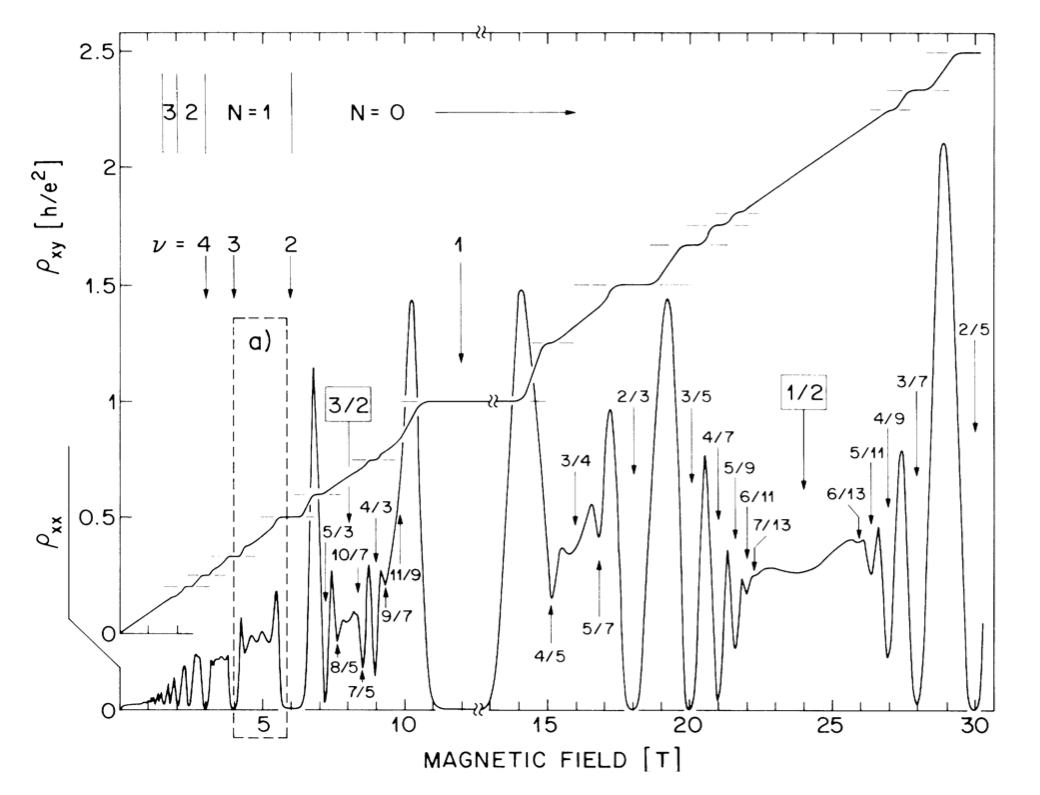
\includegraphics[width=0.9\textwidth]{figures/Introduction/FQHE.png}
    \caption{\textbf{Fractional Quantum Hall Effect} extracted from \cite{stormer1999fractional}. Fractional plateaus of transverse resistance $\rho_{xy}$ observed in GaAs/AlGaAs heterostructures at low temperatures and high magnetic fields, quantized to fractional values of $h/e^2$ at various filling factors $\nu=1/3$, $2/5$, $3/7$, etc. Note: $\nu=1/2$ is metallic --- there is no plateau at all.}
    \label{fig:FQHE}
\end{figure}
is the most famous example of a TO state, featuring fractionally charged electrons and a ground state degeneracy on the torus \cite{wen1990ground,wen1989vacuum}. In fact, it is the study of FQHE that first bought in the concept of topological orders to the condensed matter physics community, opening an era of topology in condensed matter physics that extends beyond the traditional Landau paradigm of spontaneous symmetry breaking \cite{anderson1963plasmons} (as well as renormalization group analysis) and Landau Fermi liquid theory \cite{landau1959theory}. As an intrinsic 2D systems, twisted vdW materials is much more complicated than the \emph{isotropic} electronic liquids in GaAs/AlGaAs heterostructures\footnote{In GaAs/AlGaAs heterostructures, there is always a Galinean invariance for the electronic liquids.} due to the presense of crystalline symmetries. The coexistence of symmetries and topological orders may enrich the phase diagrams, leading us to a more exotic regime of \emph{symmetry-enriched topological orders} (SET) \cite{mesaros2013classification,chen2010local}, see in Fig. \ref{fig:SPT_SET_phase_diagram}.
\begin{figure}[!htp]
    \centering
    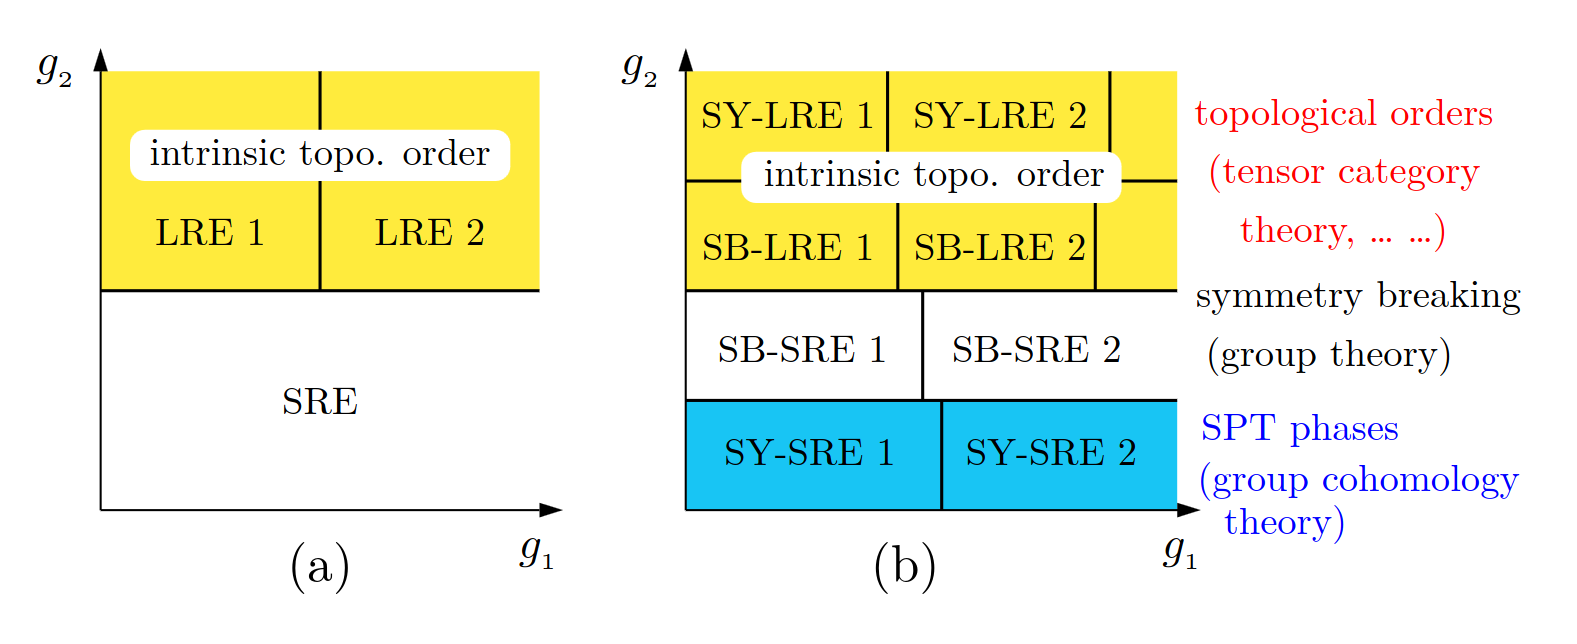
\includegraphics[width=0.8\textwidth]{figures/SPT_SET_phase_diagram.png}
    \caption{\textbf{Ilustration of Short-range Entangled and Long-range Entangled States} adapted from Ref. \cite{zeng2015quantum}. \textbf{(a)}. Possible phase diagram for a Hamiltonian $H(g_1,g_2)$ without any symmetry. \textbf{(b)}. Possible phase diagram for a Hamiltonian $H(g_1,g_2)$ with some symmetries. All shaded regions in (a) and (b) represent the phases with short range entanglement (i.e. those ground states can be
        transformed into a direct product state via a generic LU transformations that do not have any symmetry).}
    \label{fig:SPT_SET_phase_diagram}
\end{figure}

Generally speaking, twisted vdW materials stands as new platform to explore the interplay between crystalline symmetries and TO, in particular in illustration of SET states. For instance, as a significant part of this thesis, we study fractional Chern insulators (FCI), the lattice analogue of FQHE, as the interplay of intrinsic topological orders and crystalline symmetries, which is recently realized in twisted vdW materials \cite{cai2023signatures,park2023observation,lu2024fractional,zeng2023thermodynamic,xu2023observation}.


\subsection{On Moir\'e Physics}
The highlights of twisted physics is the possible formation of moiré patterns with the presence of twisting angles, which brings another long-range length scale or low-energy scale physics to the electronic system (we coin it as the \emph{moir\'e physics}). Theoretically, the effective field theory, along with Anderson's pioneering work on the declaration of independence for condensed matter physics \cite{anderson1972more}, has recognize the existence of infra-red (IR) and ultra-violet (UV) scales in each field of physics. In contrast to high-energy physics, where IR corresponds to the energy scale of the Large Hadron Collider (LHC) and UV corresponds to the unreachable Planck length related to cosmic inflation and grand unification, condensed matter physics naturally has its own IR and UV limits --- the lattice constants (short-range and high-energy) and the sample sizes (long-range and low-energy), see Fig.\ref{fig:HEP_vs_CMP}.
\begin{figure}[!htp]
    \centering
    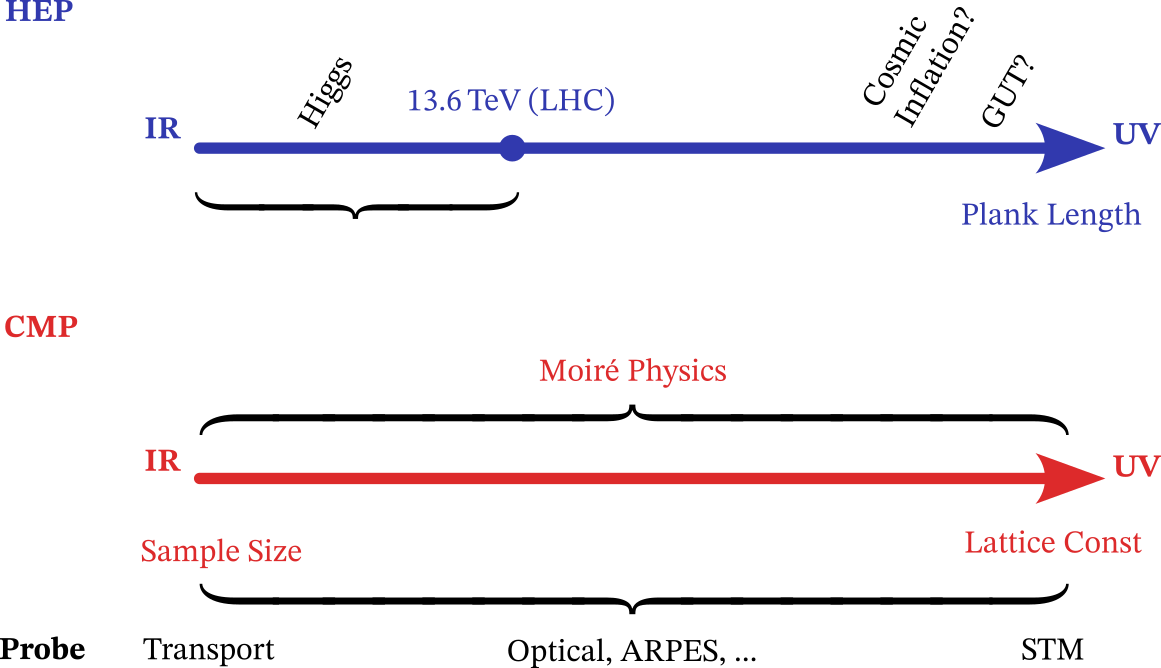
\includegraphics[width=0.6\textwidth]{figures/Introduction/HEP_vs_CMP.png}
    \caption{\textbf{UV-IR Energy Scales in High Energy and Condensed Matter Physics}.}
    \label{fig:HEP_vs_CMP}
\end{figure}

Experimentally, a natural advantage of condensed matter physics is that we can employ various kinds of probes across all energy scales. At the UV scale, we can image the electronic density of states using a scanning tunneling microscope (STM). Slightly larger than the atomic length scale, we have optical and ARPES measurements. Close to the IR limit, across the entire sample, we have transport measurements. These probes have been traditionally applied to different materials and systems. However, in twisted vdW materials, where moiré physics comes into play, although the UV details is not altered, the physical length scale can be significantly tuned with the twisting angle. This provides a unified platform for all these experimental probes to work together. The most famous example would be the significant flatten of the Dirac dispersions in twisted bilayer graphene \cite{bistritzer2011moire,cao2018correlated}. As a result, the extended tunability and the unified experimental approach provide the primary reasons why twisted physics has garnered so much attention in recent years.





\subsection{As a New Experimental Knob}
Even without moir\'e physics, twising angle itself can still serve as an extra tuning paramters along with the existing ones, including magnetic fields, gating fields, and strains. If there is a phase space of all tuning paramters, then consider twisted vdW materials is equivalent to introduce another dimension, which must be helpful for search of quantum phases, in particular for the situation when tuning other existing parameters cannot reach the target exotic phases.

For example, when considering twisted cuprates, theoretically it is proposed to have a spontaneous time-reversal symmetry (TRS) breaking when the twisting angle is close to $\theta\approx45^\circ$, giving rise to the presence of topological superconductors (TSC) phases, which is rarely realized in conventional materials, as is shown in Fig.\ref{fig:high-T_topo_SC}.
\begin{figure}[!htp]
    \centering
    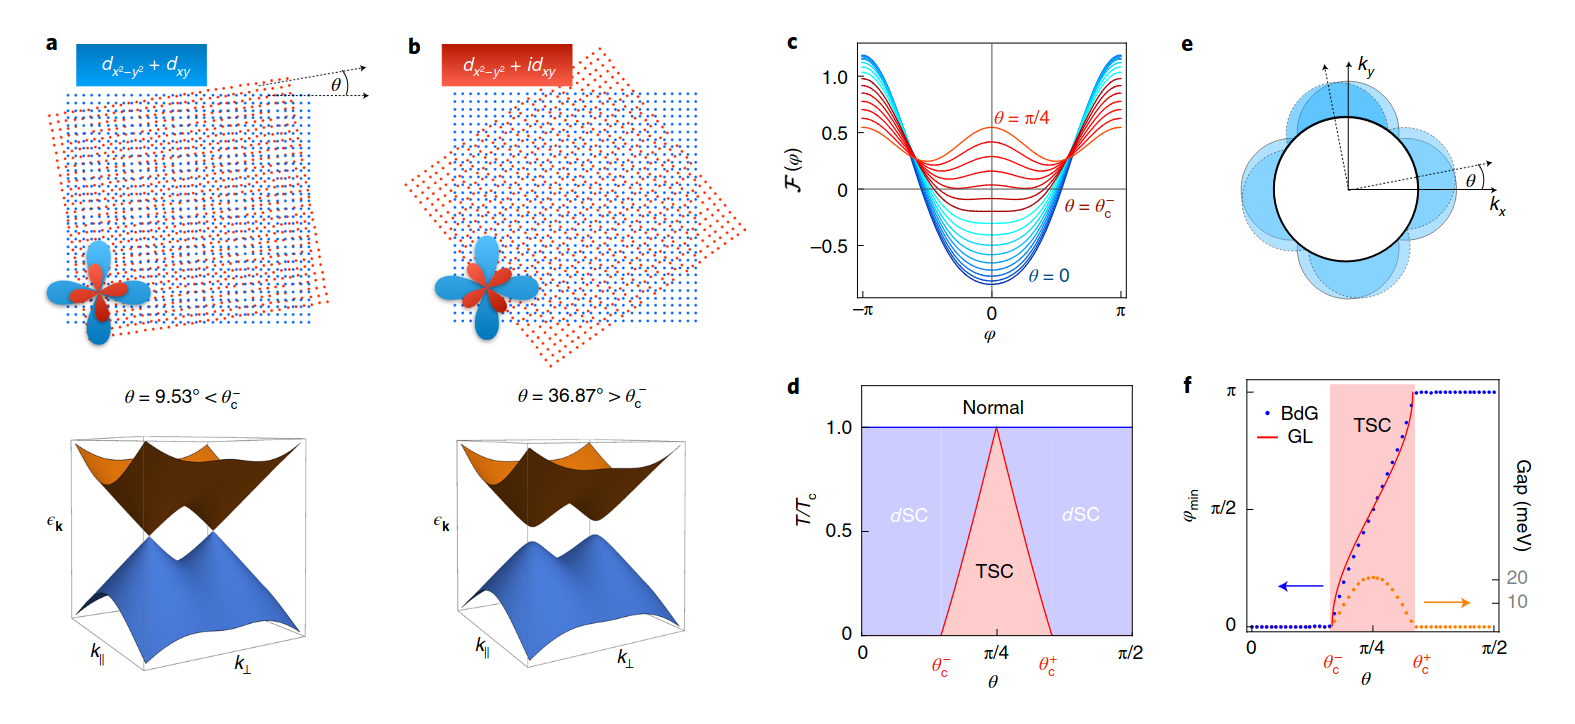
\includegraphics[width=1.0\textwidth]{figures/Introduction/high-T_topo_SC.png}
    \caption{\textbf{High-Temperature Topological Superconductors in Twisted Cuprates} extracted from Ref. \cite{can2021high}. \textbf{(a)} at small twisting angle $\theta<\theta_c$ the free energy is minimized when the interlayer phase differences $\varphi=0$, resulting in a split Dirac cone with TRS. \textbf{(b)} at large twisting angle $\theta>\theta_c$ the free energy is minimized when $\varphi\neq0$, resulting in a spontaneous TRS breaking with a fully gapped cone. \textbf{(d)} Phase diagram based on Ginzbarg-Landau free-energy analysis.}
    \label{fig:high-T_topo_SC}
\end{figure}

In a similar proposal of twisted cuprates, another group of Rutgers analysizes the node movement for small twisting angles regimes, unveil the existence of ``magic angle'' not due to moir\'e physics at all, but from the appearance of \emph{quadratic band touch point} (QBT), from which plenty of topological phase transtions can be tuned. In particular, when a vertical supercurrent is inserted, Chern number transfer would happen, leading to the realization of chiral topological superconductivity \cite{volkov2023magic,volkov2023current}. The appearance of QBT can be summazied as following:
\begin{enumerate}
    \item Two overlapped fermi surfaces, with two superconducting nodes live on them, get separated due to the interlayer tunneling $t_\perp$;
    \item The nodes get close after twisting, leading to QBT appears at some magin angle $\theta_{\text{MA}}$.
\end{enumerate}
as is illustrated Fig.\ref{fig:twisted_nodal_SC}.
\begin{figure}[!htp]
    \centering
    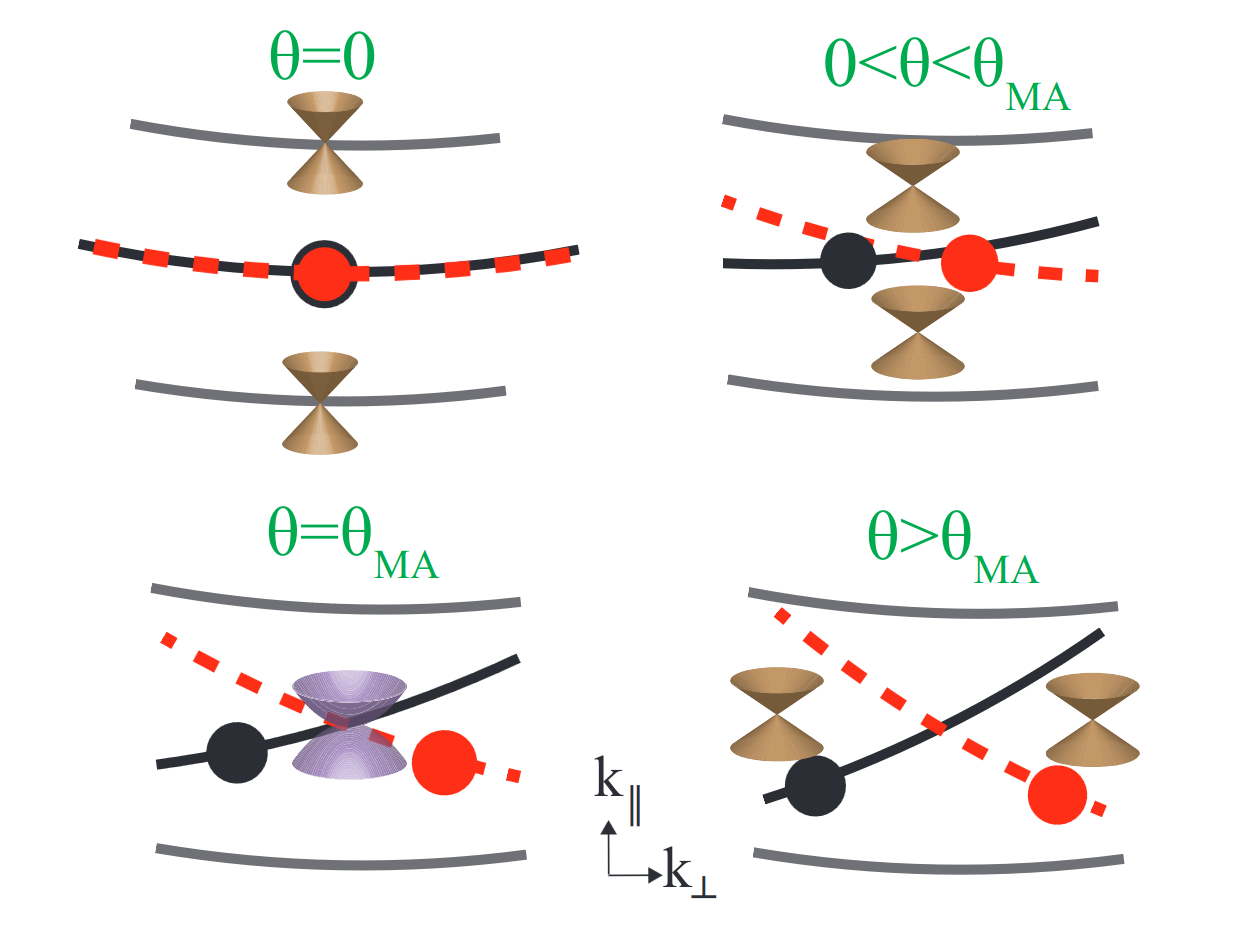
\includegraphics[width=0.6\textwidth]{figures/Introduction/node_movement.png}
    % \hspace{1em}
    % 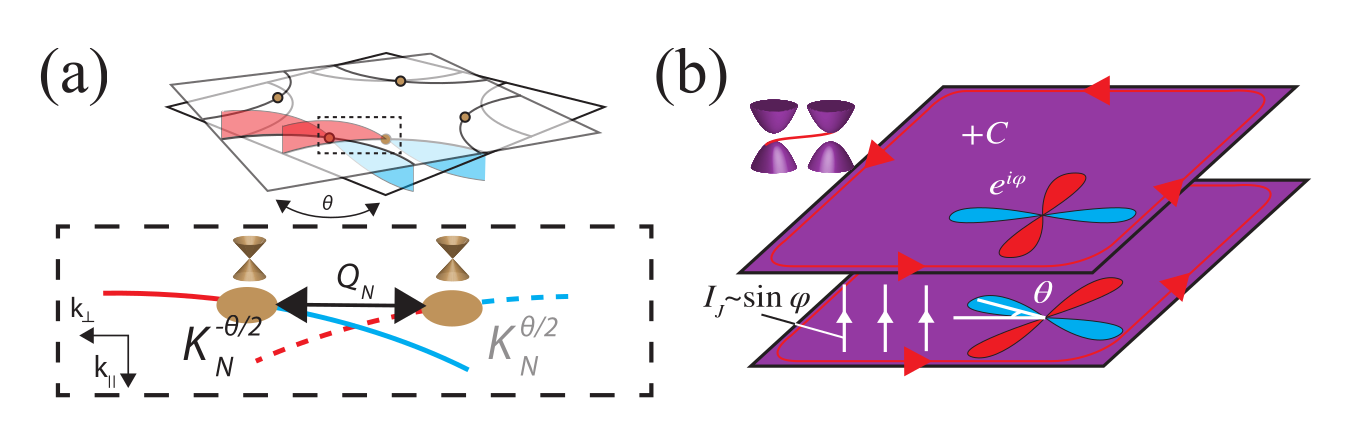
\includegraphics[width=0.45\textwidth]{figures/Introduction/pixley_twisted_nodal_SC.png}
    \caption{\textbf{Node Movement for Twisted Nodal Superconductors} adapted from Ref. \cite{volkov2023magic}. }
    \label{fig:twisted_nodal_SC}
\end{figure}


\subsection{As a Platform for Quantum Simulations}
As is discussed before, the unique feature for the platform of twisted vdW materials is the possible presence of the moir\'e physics. The size of Moir\'e patterns are tightly connected with the twisting angles, so can be used to cover a wide range of physical length/energy scales, which can be useful for searching of more exotic phases.

The most famous example, as a declaration on the born of twisted physics (or twistronics), is the dicovery of correlated insulating phases and unconventional superconductivity in twisted bilayer graphene (tBLG) \cite{cao2018correlated,cao2018unconventional}, as is shown in Fig.\ref{fig:tBLG_SC_Cao}. Although the superconducting transition temperature seems to be low in tBLG, it indeed falls into the strongly-correlated regime\footnote{Actually tBLG is more strongly-correlated in comparison with cuprates.} because of its much lower carrier density in the moir\'e superlattice (around $1.0\times 10^{12}$ cm$^{-2}$ compared to the cuprates around $1.0\times10^{14}$ cm$^{-2}$).
\begin{figure}[!htp]
    \centering
    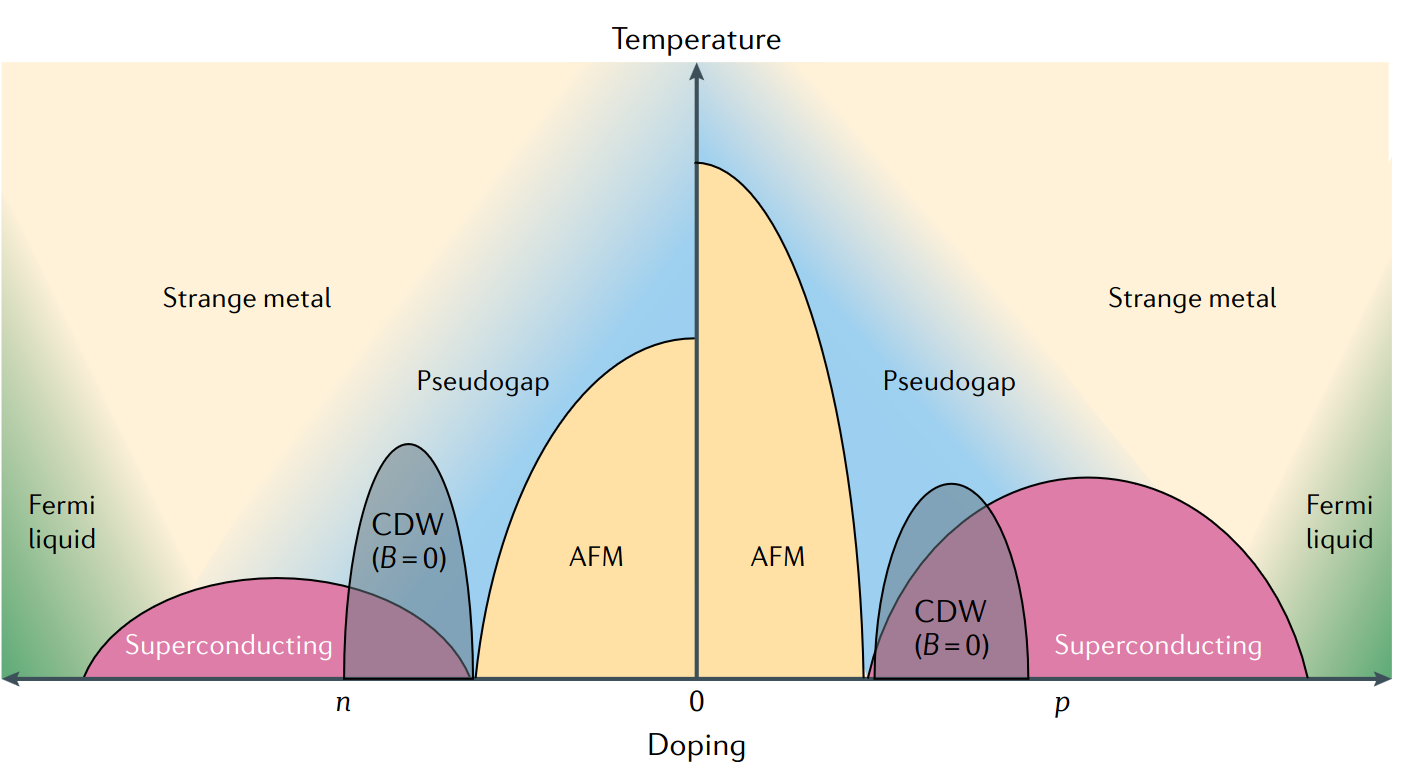
\includegraphics[height=0.32\textwidth]{figures/Introduction/high_Tc_SC_phase_diagram.png}
    \hspace{1em}
    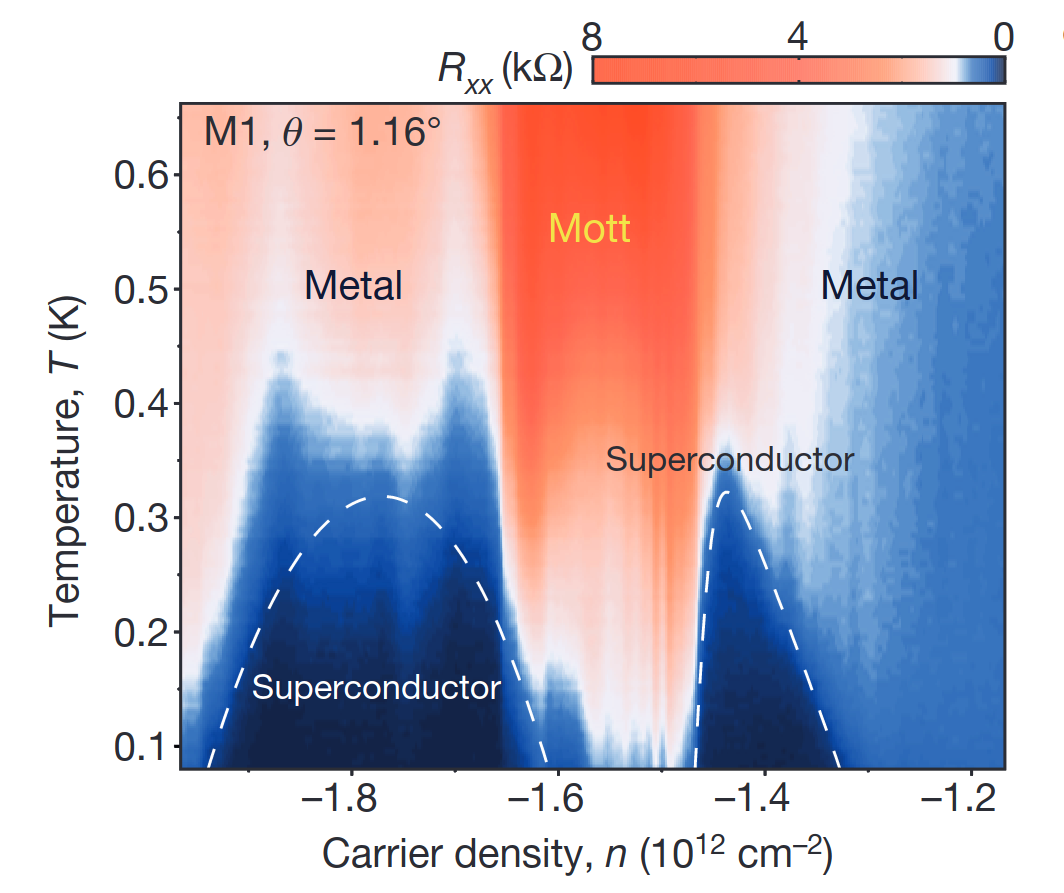
\includegraphics[height=0.32\textwidth]{figures/Introduction/tBLG_SC_Cao_new.png}
    \caption{\textbf{Phase Diagram for the Unconventional Superconductivity} extracted from Ref. \cite{zhou2021high} and Ref. \cite{cao2018unconventional}. The superconducting domes adjacent to mott insulating phase is similar in cuprates phase diagram (left) and tBLG phase diagram (right).}
    \label{fig:tBLG_SC_Cao}
\end{figure}
Thereafter, extensive work of correlated physics around the superconducting phases has been studied in tBLG, including the competing orders like nematicity \cite{cao2021nematicity}, and the linear-$T$ resistivity in strange metals \cite{cao2020strange}. Outside of superconductivity, there are other correlated phenomena, including the ferromagnetism \cite{sharpe2019emergent}, quantum anomalous Hall effect \cite{serlin2020intrinsic}, and even the fractional chern insulators \cite{xie2021fractional} (still with small external magnetic fields, though) has been found in tBGL, see Fig.\ref{fig:tBLG_FQHE}.
\begin{figure}[!htp]
    \centering
    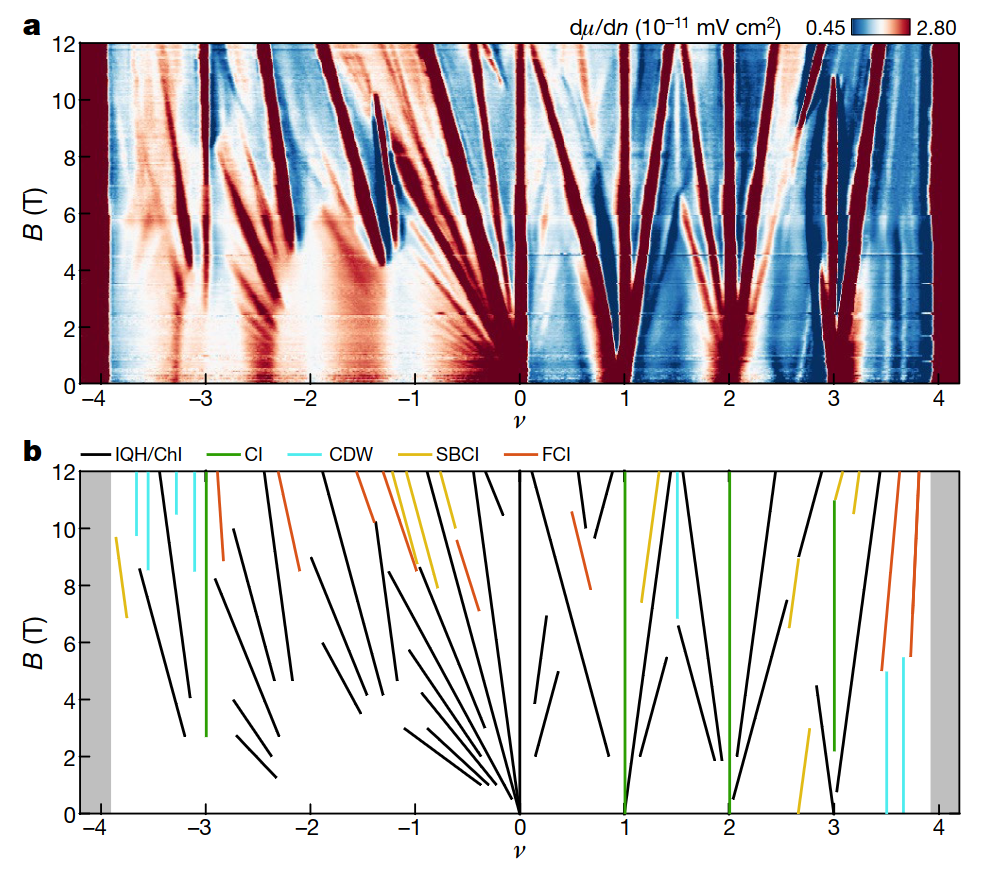
\includegraphics[width=0.75\textwidth]{figures/Introduction/tBLG_FQHE.png}
    \caption{\textbf{Fractional Chern Insulators in tBLG} adapted from Ref.\cite{xie2021fractional}. Streda formula $C=\frac{\partial n}{\partial B}$ can be used to extract the states. Here $\nu$ is the number of electrons per moir\'e unit cell, and the FCI states are those that possess both fractional slopes and fractional interceptions.}
    \label{fig:tBLG_FQHE}
\end{figure}



Apart from graphene, the huge family of transition metal dichalcogenides (TMDs) also provide other choices for the building blocks of twisted 2D vdW materials. Correlated phases like mott insulators can still be realized \cite{zhang2020flat,wang2020correlated} in twisted TMD, as flat bands are also reproducible either due to moir\'e physics or lattice relaxation \cite{devakul2021magic,li2021lattice}. But more imporantly,  due to the more complicated electronic band structures \cite{manzeli20172d} and extra controllable knobs like valley/spin degrees of freedom \cite{xiao2012coupled}, the twisted TMD platform can be expected to realize more exotic phases. The most convincing example would be the realization on the phase of fractional Chern insulators (FCI), which is numerically heavily studied one decade ago \cite{neupert2011fractional,tang2011high,sheng2011fractional,regnault2011fractional}, as a natural theoretical extension of FQHE on lattices, but has never be realized in experiments until last year (2023), when three independently groups in UW \cite{cai2023signatures,park2023observation}, Cornell \cite{zeng2023thermodynamic}, and SJTU \cite{xu2023observation} claim the observation of fractional quantum anomalous Hall effect (FQAH) in twisted MoTe$_2$ (tMoTe$_2$), as is show in Fig. \ref{fig:tMoTe2_UW}.
\begin{figure}[!htp]
    \centering
    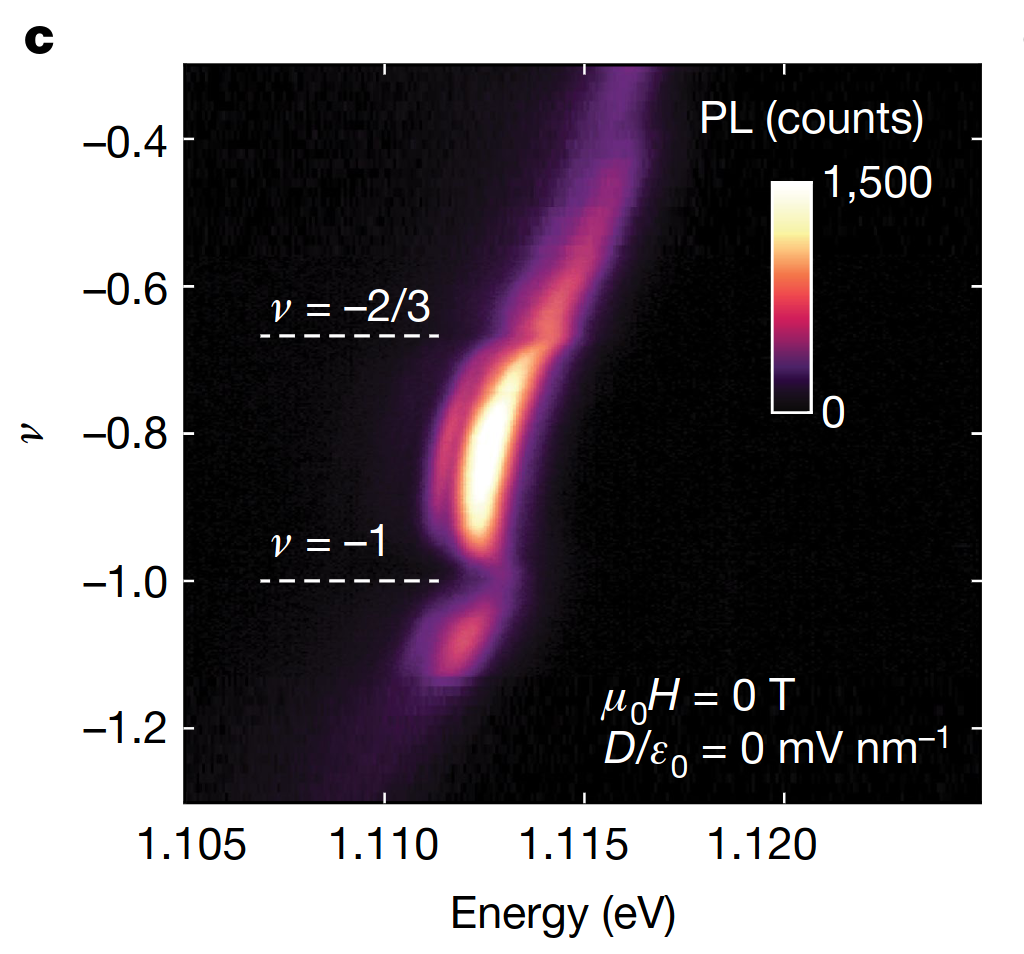
\includegraphics[height=0.4\textwidth]{figures/Introduction/tMoTe2_PL.png}
    \hspace{1em}
    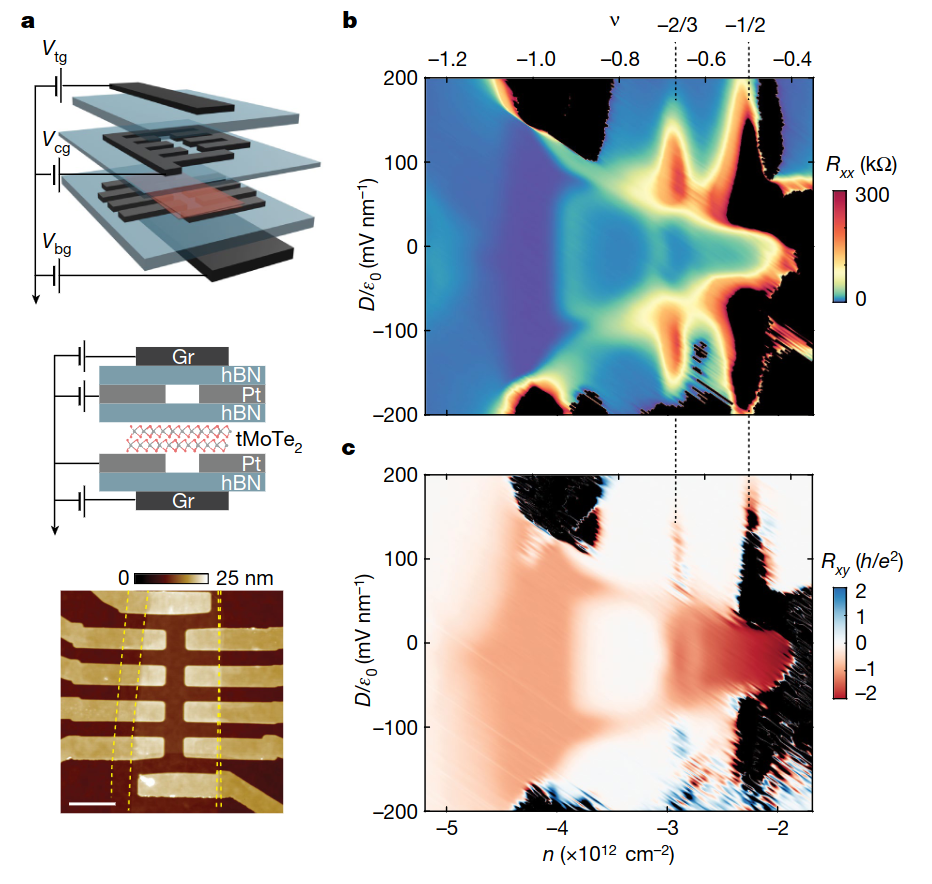
\includegraphics[height=0.4\textwidth]{figures/Introduction/tMoTe2_transport.png}
    \caption{\textbf{Experimental Obverservation of Fractional Quantum Anomalous Hall Effects in tMoTe$_2$} extracted from Ref. \cite{cai2023signatures} (left) and Ref. \cite{park2023observation} (right).}
    \label{fig:tMoTe2_UW}
\end{figure}
As another interesting fact, fractional quanutum anomalous Hall effects are also realized in rhombohedral pentalayer graphene (RPG)-hBN moir\'e superlattice very recently in MIT group \cite{lu2024fractional}, exhibiting the power of both stacking and twisting engineerings.



\section{Structure of the Thesis}
In this thesis, I will focus on the study of the quantum phases of matter in two-dimensional space, particularly in the context of the twisted 2D vdW materials exhibiting complexities from the interplay of symmetry, topology (either free-fermion topology or in the sense of topological orders), and strong correlations. The thesis is organized as follows:
\begin{itemize}
    \item In the first (this) chapter, I briefly discuss the motivation for studying the twisted 2D vdW materials, from the perspective of both experimental feasibility and theoretical complexity. Due to the unique features of moir\'e physics, twisted 2D vdW materials appears as the new platform for exploring exotic quantum phases of matter.
    \item In the second chapter, to make the thesis self-contained, I will introduce some necessary background, stating from simple $\bm k\cdot\bm p$ analysis of graphene and transition metal dichalcogenides (TMD) to a general derivation for the moir\'e continuum Hamitonian. This chapter will also include the basic knowledge of fractional quantum Hall effect (FQHE), in particular the vortex-binding picture of composite fermions (CF), and some previous theoretical efforts on mapping fractional Chern insulators (FCI) states to the lowest Landau levels (LLL).
    \item As the main part of the thesis, I will list three of my works on twisted 2D vdW materials:
          \begin{itemize}
              \item The first long and recent work is for fractional Chern insulators, the lattice analogue of FQHE, realized in recent experiments. To adress many fundamental questions closely related to the microscopic understandings of FCI, We propose a projective construction based on Murthy-Shankar's CFs. The construction mainly splits into four steps: a Chern band to LLL mapping, the CF substituion on lattice, a CF mean-field state and computation of CF excitations (as magnetorotons), and the electronic projections. In construction of the framework, all factors of complexity mentioned above get intertwined, including moir\'{e} physics, strong correlations, and symmetry-enriched topological orders.
              \item The last two works are about twisted 2D superconductors in small twisting angle regime. The first work is to extend the picture of topological phase transitions in twisted cuprates to twisted Ising superconductors like NbSe$_2$ and TaS$_2$, to give another platform for realization of chiral topological superconductivity. The second work is to take the twisted 2D superconductors as a general platform for transport measurements breaking, where we propose the supercurrent-induced anomalous thermal Hall effects as a sharp probe to the superconducting gap anisotropy.
          \end{itemize}
\end{itemize}



% \section{Twisted with Moir\'e Physics: Twisted TMD}
% \section{Twisted without Moir\'e Physics: Twisted Cuprates}